% LaTeX Präsentationsvorlage (2013) der TU Graz, rev12, 2013/01/31
\documentclass{beamer}
% \documentclass[aspectratio=169]{beamer}
% \usetheme{tugraz2013}
% \usetheme[notes]{tugraz2013}
\usetheme{tugraz2013}
\usepackage{color}
\usepackage{multicol}
\usepackage{bbding}
\usepackage{wasysym}

\usepackage{picture}
\usepackage{rotating}

\definecolor{darkred}{rgb}{0.85,0.16,0.0}
\definecolor{darkgreen}{rgb}{0.16,0.70,0.27}

\newcommand{\red}[1]{{\color{red} #1}}
\newcommand{\blue}[1]{{\color{blue} #1}}
\newcommand{\darkgreen}[1]{\textcolor{darkgreen}{#1}}
\newcommand{\darkred}[1]{\textcolor{darkred}{#1}}

\newcommand*{\vpointer}{\vcenter{\hbox{\scalebox{1.5}{\large\pointer}}}}

\newcommand{\be}[1]{\begin{equation} \label{#1}}
\newcommand{\ee}{\end{equation}}
\newcommand{\bea}[1]{\begin{eqnarray} \label{#1}}
\newcommand{\eea}{\end{eqnarray}}
\newcommand{\bean}{\begin{eqnarray*}}
\newcommand{\eean}{\end{eqnarray*}}

\newcommand{\non}{\nonumber\\}
\newcommand{\eq}[1]{(\ref{#1})}
\newcommand{\difp}[2]{\frac{\partial #1}{\partial #2}}
\newcommand{\br}{{\bf r}}
\newcommand{\bR}{{\bf R}}
\newcommand{\bA}{{\bf A}}
\newcommand{\bB}{{\bf B}}
\newcommand{\bE}{{\bf E}}
\newcommand{\bm}{{\bf m}}
%\renewcommand{\bm}{{\bf m}}
\newcommand{\bn}{{\bf n}}
\newcommand{\bN}{{\bf N}}
\newcommand{\bp}{{\bf p}}
\newcommand{\bP}{{\bf P}}
\newcommand{\bF}{{\bf F}}
\newcommand{\by}{{\bf y}}
\newcommand{\bz}{{\bf z}}
\newcommand{\bZ}{{\bf Z}}
\newcommand{\bV}{{\bf V}}
\newcommand{\bv}{{\bf v}}
\newcommand{\bu}{{\bf u}}
\newcommand{\bx}{{\bf x}}
\newcommand{\bX}{{\bf X}}
\newcommand{\bW}{{\bf W}}
\newcommand{\bJ}{{\bf J}}
\newcommand{\bj}{{\bf j}}
\newcommand{\bk}{{\bf k}}
\newcommand{\bTheta}{{\bf \Theta}}
\newcommand{\btheta}{{\boldsymbol\theta}}
\newcommand{\bOmega}{{\bf \Omega}}
\newcommand{\bomega}{{\boldsymbol\omega}}
\newcommand{\brho}{{\boldsymbol\rho}}
\newcommand{\rd}{{\rm d}}
\newcommand{\rJ}{{\rm J}}
\newcommand{\ph}{{\varphi}}
\newcommand{\te}{\theta}
\newcommand{\tht}{\vartheta}
\newcommand{\vpar}{v_\parallel}
\newcommand{\vparkb}{v_{\parallel k b}}
\newcommand{\vparkm}{v_{\parallel k m}}
\newcommand{\Jpar}{J_\parallel}
\newcommand{\ppar}{p_\parallel}
\newcommand{\Bpstar}{B_\parallel^*}
\newcommand{\intpi}{\int\limits_{0}^{2\pi}}
\newcommand{\summ}{\sum \limits_{m=-\infty}^\infty}
\newcommand{\tb}{\tau_b(\uv)}
\newcommand{\bh}{{\bf h}}
\newcommand{\cE}{{\cal E}}
\newcommand{\bsigma}{{\boldsymbol\sigma}}
\newcommand{\bS}{{\mathbf S}}
\newcommand{\bI}{{\mathbf I}}
\newcommand{\odtwo}[2]{\frac{\rd #1}{\rd #2}}
\newcommand{\pdone}[1]{\frac{\partial}{\partial #1}}
\newcommand{\pdtwo}[2]{\frac{\partial #1}{\partial #2}}
\newcommand{\ds}{\displaystyle}

%% Titelblatt-Einstellungen
\title[]
{Geometric Integration of \\Guiding Center Orbits in Magnetically Confined Plasmas and Applications}
\author[L.~Bauer]{\scriptsize Lukas Bauer, BSc. \\
	Institute of Theoretical and Computational Physics - Plasma Physics\\Group of Prof. W. Kernbichler (Graz University of Technology)
}
\date{10. July 2020, Seminar Presentation, Graz} % \today für heutiges Datum verwenden
%\date{\today}
\institute[Institute of Theoretical and Computational Physics]
{
}
\instituteurl{www.tugraz.at}
% \institutelogo{kurz.pdf}
\additionallogo{merged_logos_m.png}

%%%%%%%%%%%%%%%%%%%%%%%%%%%%%%%%%%%%%%%%%%%%%%%%%%%%%%%%%%%%%%%%%%%%%%%%%%%%
\begin{document}
%	\setbeameroption{show notes}% un-comment to see the notes
%%%%%%%%%%%%%%%%%%%%%%%%%%%%%%%%%%%%%%%%%%%%%%%%%%%%%%%%%%%%%%%%%%%%%%%%%%%%
\titleframe

%\begin{frame}
%  \frametitle{Outline}
%  \tableofcontents%[hideallsubsections] 
%  \note{
%  	Meine Präsentation ist wie folgt strukturiert \ldots
%  }
%\end{frame}

\section{Introduction}
% \begin{frame}
% \begin{center}
% \vfill
% {\Large Motivation}
% \vfill
% \end{center}
% \end{frame}








\section{Kinetic equilibria}
%\sectionheader[M. Eder, C.G. Albert, S.V. Kasilov, W. Kernbichler]{Three-dimensional geometric integrator for charged particle orbits in toroidal fusion devices}

\begin{frame}
\frametitle{Computation of kinetic equilibria}
\begin{itemize}
\item Kinetic modelling of edge plasmas
\item Quasi-steady plasma parameters in 3D toroidal fusion devices
\begin{itemize}
\item Simple (cylindrical) modelling of perturbed tokamak equilibria shows that the problem of shielding of external perturbations is essentially kinetic.
\item 3D equilibria should be computed by using plasma response currents and charges in kinetic approximation. \\
$\rightarrow$ Global Monte Carlo modelling
\end{itemize}
\end{itemize}
\end{frame}

%\begin{frame}
%\frametitle{Global Monte Carlo modelling}
%\begin{itemize}
%\item The purpose is integration of guiding center orbits for Monte Carlo evaluation of plasma response to external non-axisymmetric perturbations from ELM mitigation coils. 
%\item Namely, this is the perturbed pressure tensor, parallel current and charge density needed for iterative solution of Maxwell equations within kinetic modelling of plasma equilibrium.
%\end{itemize}
%\end{frame}

\begin{frame}
\frametitle{Modelling of kinetic equilibria}
%\vspace{-1.5cm}
	\centering 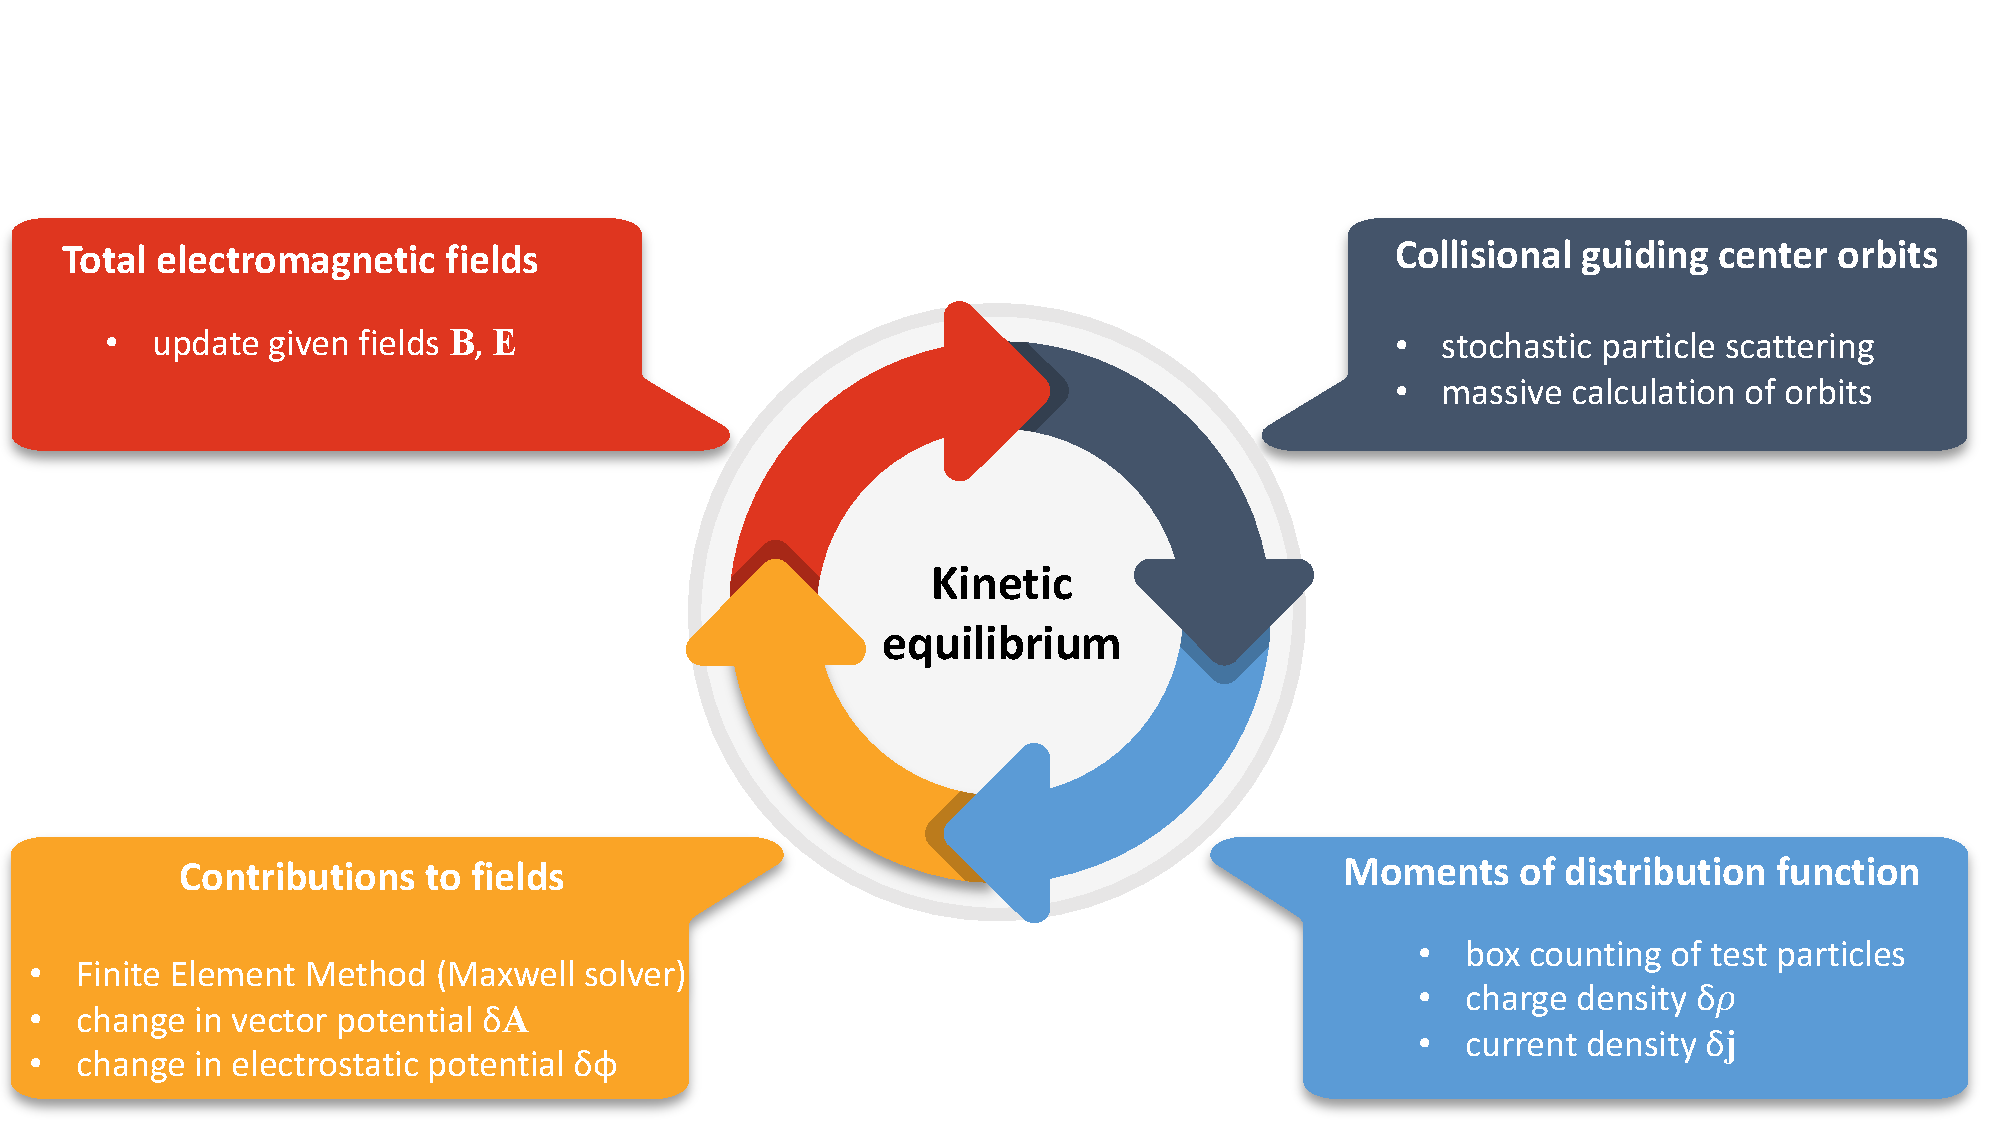
\includegraphics[trim={0 0 0 3cm},clip,width=\textwidth]{FIGURES/cycle01.pdf}
\end{frame}


\begin{frame}[noframenumbering]
\frametitle{Modelling of kinetic equilibria}
%\vspace{-1.5cm}
	\centering 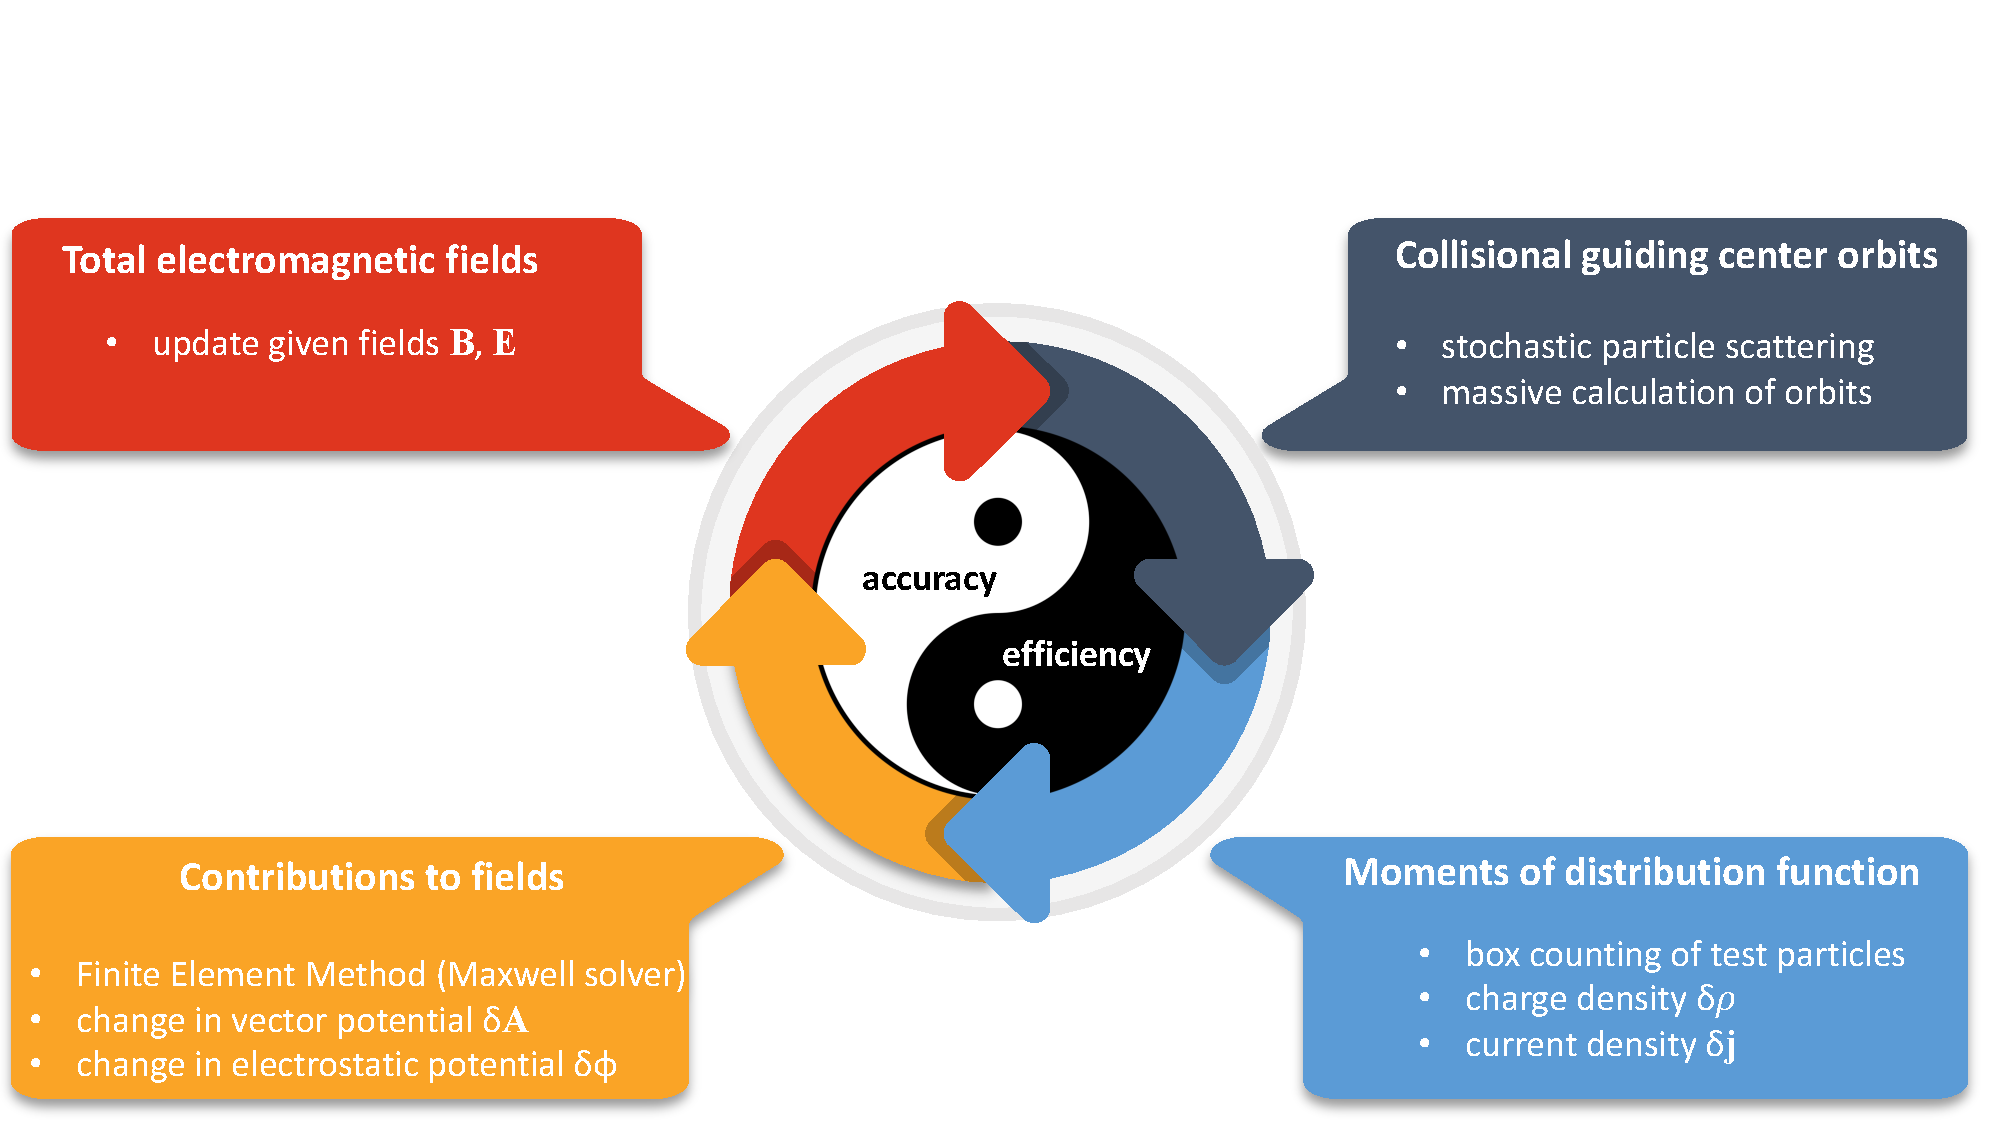
\includegraphics[trim={0 0 0 3cm},clip,width=\textwidth]{FIGURES/cycle02.pdf}
\end{frame}






\begin{frame}
\frametitle{Requirements to orbit integrator}
\begin{enumerate}
\item \textbf{Physically correct long time orbit dynamics}
\item \textbf{Low sensitivity to noise in fields:} Perturbation field from plasma response currents and charges is noisy due to stochasticity of particle collisions (Monte Carlo).
\item \textbf{Integrator efficiency:} Millions of orbits should be followed for few collision times at each iteration.
\item \textbf{Efficient box counting:} Orbit intersections with boundaries of grid cells should be traced efficiently.

\end{enumerate}
\end{frame}

\section{3D Geometric Integrator}

\begin{frame}
\frametitle{3D geometric integrator properties}
\begin{itemize}
	\item \textbf{Physically correct long time orbit dynamics}
	\begin{itemize}
		\item preserved total energy
		\item preserved magnetic moment
		\item preserved phase space volume 
	\end{itemize}
	\item \textbf{Computationally efficient:} Relaxed requirements to the accuracy of guiding center orbits
		\begin{itemize}
			\item not exact orbit shape
			\item not exact time evolution
		\end{itemize}
\end{itemize}
\end{frame}

\begin{frame}
\frametitle{Formulation of the geometric integrator}
\note{Guiding center equations!! Talk about linearizations, explain that we have 4 independent phasespace variables}
\vspace{-0.5cm}
Use the Hamiltonian form of guiding center equations in curvilinear coordinates,
\be{eqm_curv}
\dot x^i = \frac{v_\parallel \varepsilon^{ijk}}{\sqrt{g} B_\parallel^\ast}\difp{A^\ast_k}{x^j}, \qquad A^\ast_k = A_k + \frac{v_\parallel}{\omega_c}B_k,
\ee
\be{}
v_\parallel=\sigma \left(\frac{2}{m_\alpha}\left(w-J_\perp\omega_c-e_\alpha\Phi\right)\right)^{1/2}.
\ee
\vspace{0.2cm}\\
Approximate $A_k, B_k/ \omega_c$, $\omega_c$ and $\Phi$ by linear functions in spatial cells with equations of motion
\be{standeqset}
\frac{\rd z^i}{\rd \tau} = a^i_k z^k + b^i.
\ee
\end{frame}


\begin{frame}
\frametitle{3D field aligned grid: tetrahedral cells}
\vspace{-1.7cm}
%\hspace{-7cm}
	\begin{figure}
		\hspace*{-1.65cm}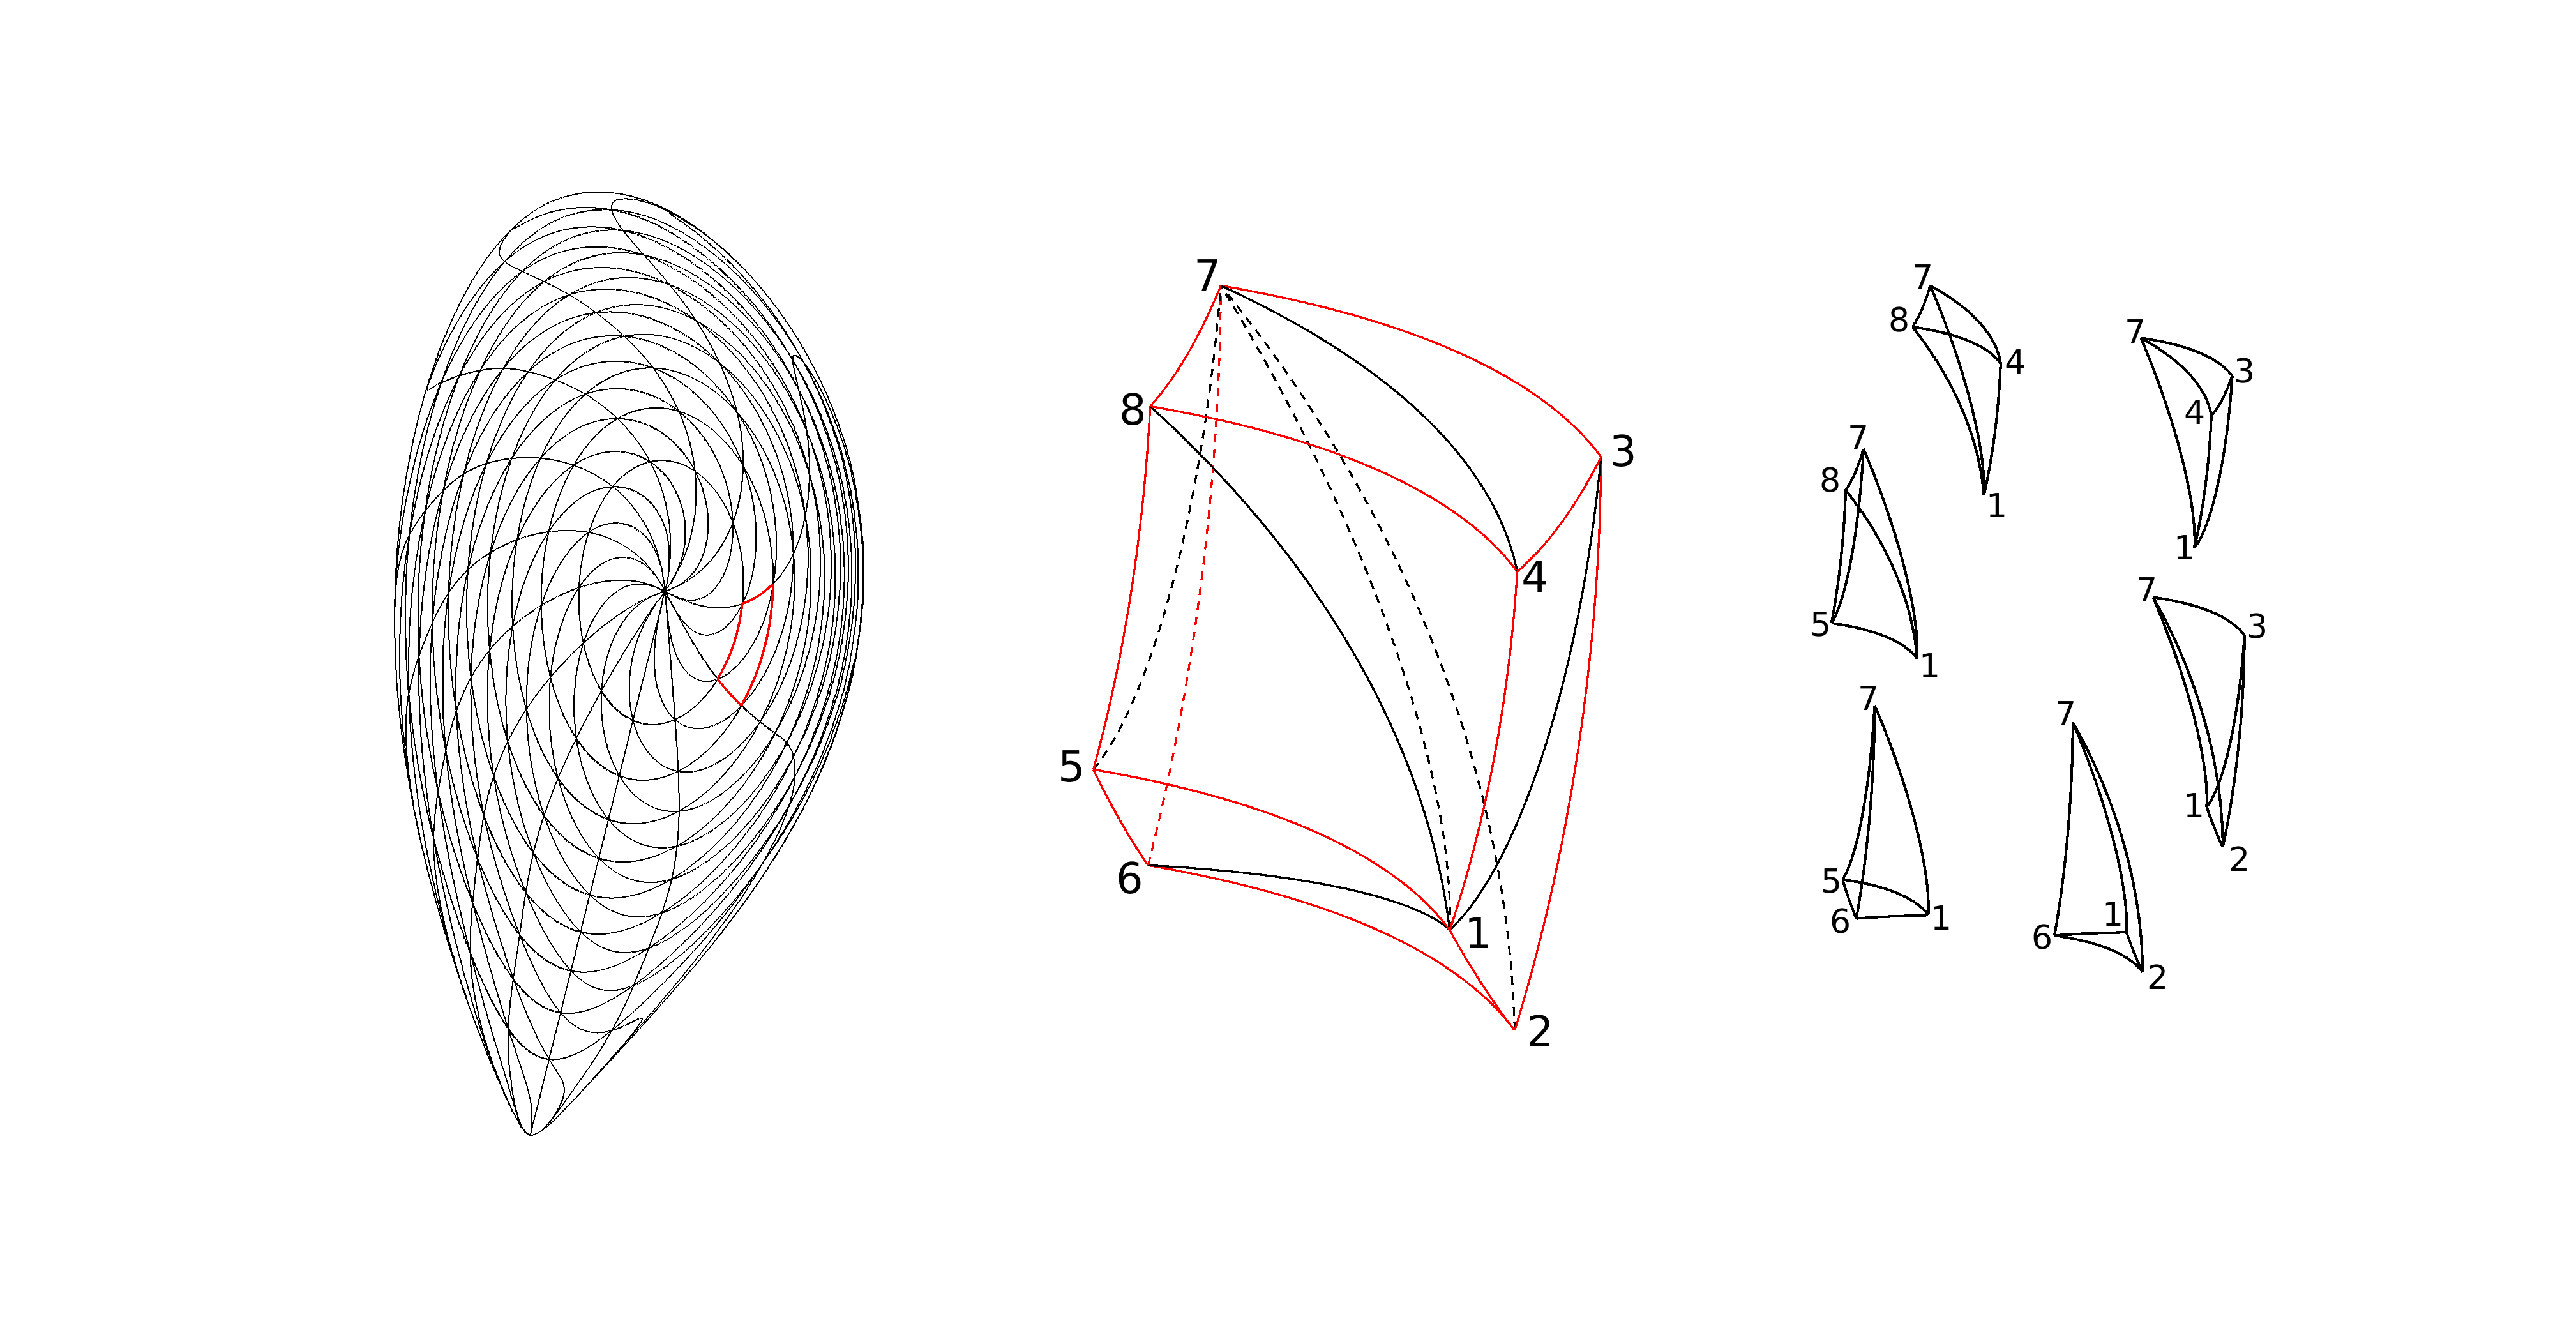
\includegraphics[width=1.25\textwidth]{FIGURES/curvilinear_grid.eps}
	\end{figure}

\end{frame}

\section{Meeting the requirements}

\begin{frame}
\frametitle{Physically correct long time orbit dynamics}
\vspace{-0.5cm}
\begin{itemize}
	\item
	Linear approximation of field quantities does \textbf{not destroy the Hamiltonian nature} of the original guiding center equations.
	\item Non-canonical Hamiltonian form of linear ODE set
	\be{hamform}
	\frac{\rd z^i}{\rd \tau}=\Lambda^{ij}\difp{H}{z^j}, \qquad \Lambda^{ij}(\bz)=\left\{z^i,z^j\right\}_\tau,
	\ee
	with Hamiltonian $H(\bz)=v_\parallel^2/2-U(\bx)$ and antisymmetric Poisson matrix  $\Lambda^{ij}(\bz)$.
	\item \textbf{Symplecticity:} Phase space volume is conserved.
\end{itemize}

\end{frame}

\begin{frame}
\frametitle{Computational method - efficiency}
\vspace{-0.5cm}
\begin{itemize}
	\item Piecewise-constant coefficients of 
	$$
	\frac{\rd z^i}{\rd \tau} = a^i_k z^k + b^i
	$$
	are discontinuous at cell boundaries. 
	\item Orbit intersections with tetrahedra faces must be computed exactly when integrating particle trajectories.
	
	\item The ODE set is numerically solved via \textbf{Runge-Kutta~4} in an iterative scheme.
	\item Iterative scheme uses \textbf{Newton's method} and a parabolic analytic estimation for the  initial step length.
\end{itemize}
\end{frame}

\begin{frame}
\frametitle{Error of the RK~4 method}
\vspace{-0.5cm}
\begin{itemize}
	\item The relative integration error of a single step between cell boundaries strongly \textbf{scales with the Larmor radius $\rho$}.
	
	\item The error is in the order of
	\be{RK4estimation}
	\frac{\delta R(\Delta\tau)}{a} \sim \frac{\rho^3}{q^4 R^3} \Delta \varphi^5,
	\ee
	with $R$, $a$, $q$ and $\Delta\varphi$ denoting major radius, plasma radius, safety factor and toroidal cell length.
	
	\item 
	The \textbf{error of the RK4 method} can be brought \textbf{below computer accuracy}.
\end{itemize}
\end{frame}

\begin{frame}
\frametitle{Poincare plots of guiding center orbits}
\note{Alles erklaeren}
\vspace{-1.1cm}
%\hspace{-7cm}
\begin{figure}
	\hspace*{-0.9cm}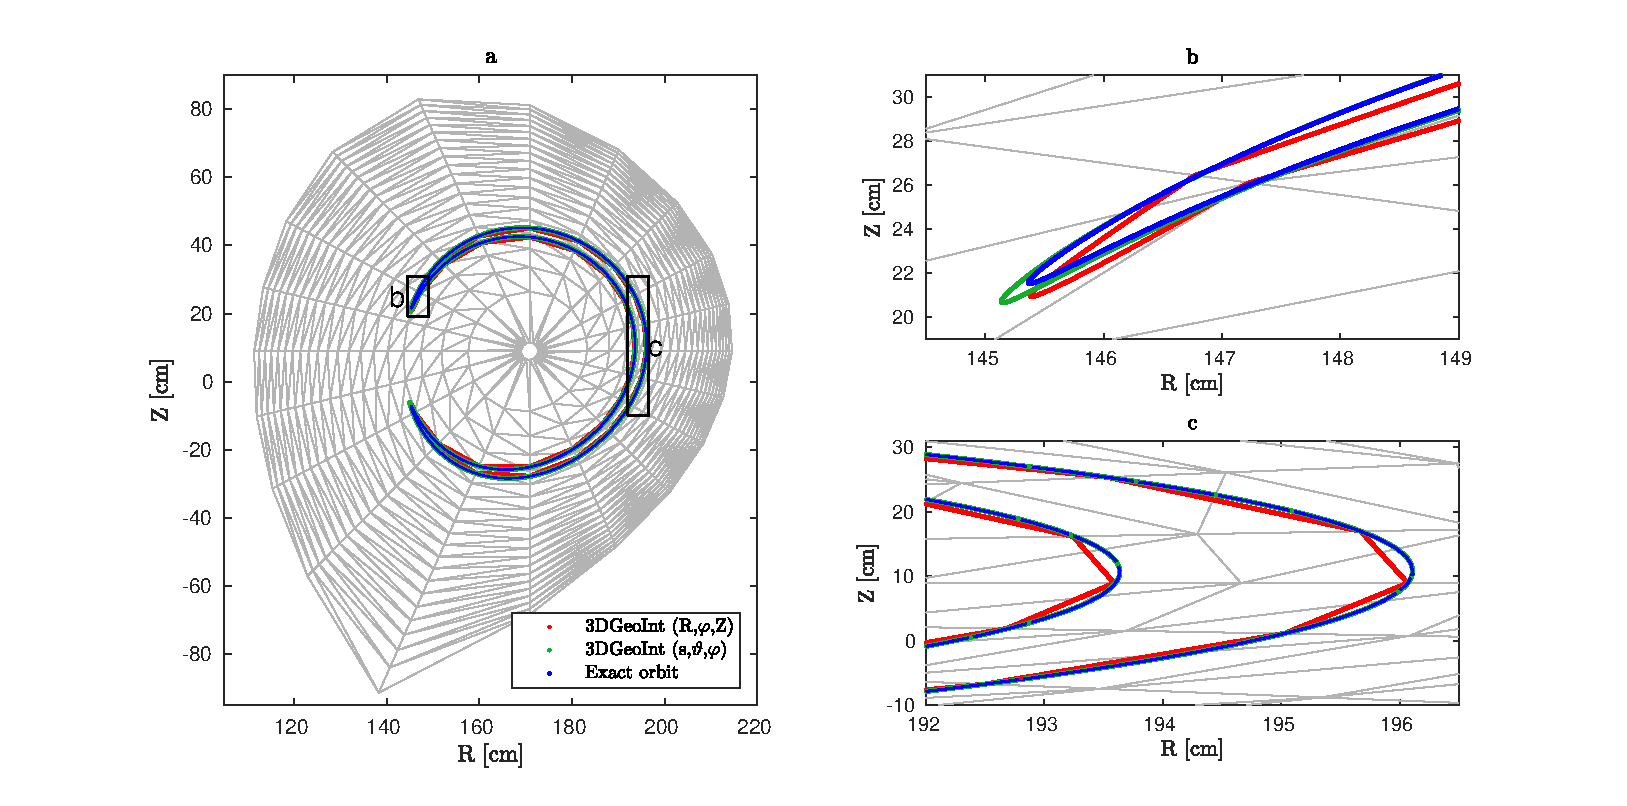
\includegraphics[width=1.0\textwidth]{FIGURES/orbit_plot.eps}
\end{figure}
\begin{itemize}
	\vspace*{-0.5cm}
\item Geometric integration: Not exact orbit shape.
\item Axisymmetic (2D): Canonical toroidal angular momentum is preserved.
\end{itemize}
\end{frame}

\begin{frame}
\frametitle{Axisymmetric noise of electrostatic and vector potential}
\vspace{-0.4cm}
%\hspace{-7cm}
\begin{figure}
	\hspace*{-1.05cm}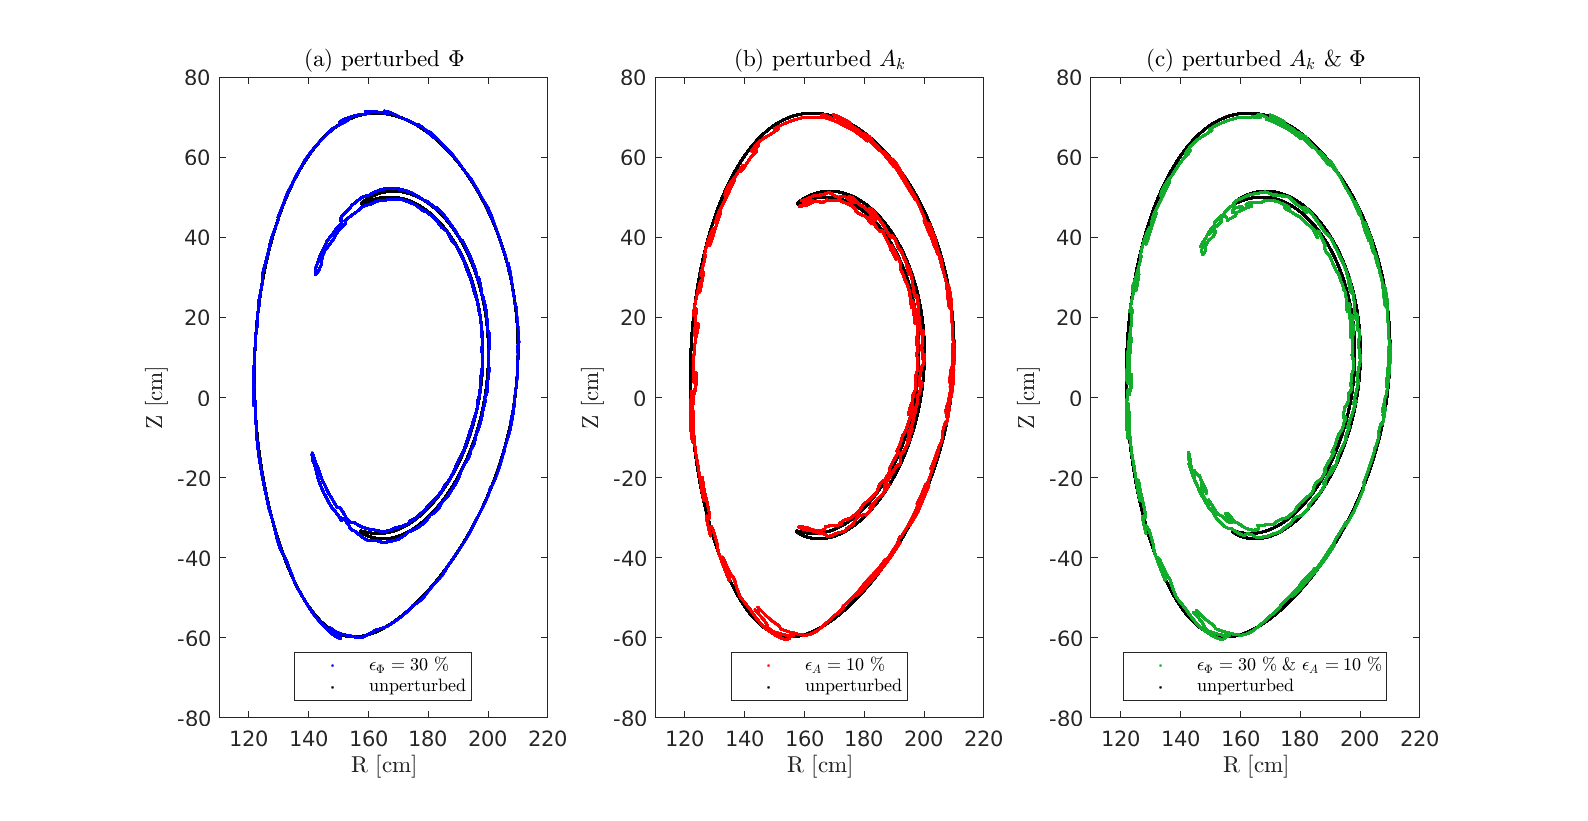
\includegraphics[width=1.0\textwidth]{FIGURES/axissymetric_noise.eps}
\end{figure}
\begin{itemize}
	\vspace*{-0.6cm}
	\item Similar orbit shape (compared to unperturbed orbit)
	\item Canonical toroidal angular momentum is preserved.
\end{itemize}
\end{frame}

\section{Artifact: Numerical diffusion}

\begin{frame}
\frametitle{Artifact: Numerical field line diffusion}
\vspace{-0.5cm}
\begin{itemize}
\item
Due to the linearization of fields for 3D configurations, \textbf{KAM surfaces do not exist anymore}. \\
$\rightarrow$ \textbf{ergodic passing particle orbit}
\item This behaviour is\textbf{ diffusive} and its
variance can be described by a field line diffusion coefficient $D_M^{ss}$ as
$\left\langle \delta s^2\right\rangle=2 D_M^{ss} N$ where $N$ is the number of toroidal orbit turns.
\item \textbf{Strong inverse scaling} of \textbf{$D_M^{ss}$ with poloidal $N_\vartheta$ and toroidal $N_\varphi$ grid sizes}, which roughly agrees with 
\be{quasilinear_diffco}
D^{ss}_M = \frac{2 \pi^2}{3} \left( \frac{\psi_{\text{pol}} \epsilon_M }{\psi_{\text{tor}}^a}\right)^2 \frac{q^4 m_0^2 n_0^2 
	\left(m_0 N_\vartheta + n_0 N_\varphi \right)^2}{N_\vartheta^2 N_\varphi^2 \left( q N_\varphi-N_\vartheta\right)^2}.
\ee
\vspace{-1cm}
\tiny{(quasilinear theory)}
\vspace{1cm}
\end{itemize}
\end{frame}


\begin{frame}
\frametitle{Artifact: Numerical field line diffusion}
\vspace{-1.4cm}
%\hspace{-7cm}
\begin{figure}
\hspace*{-1.4cm}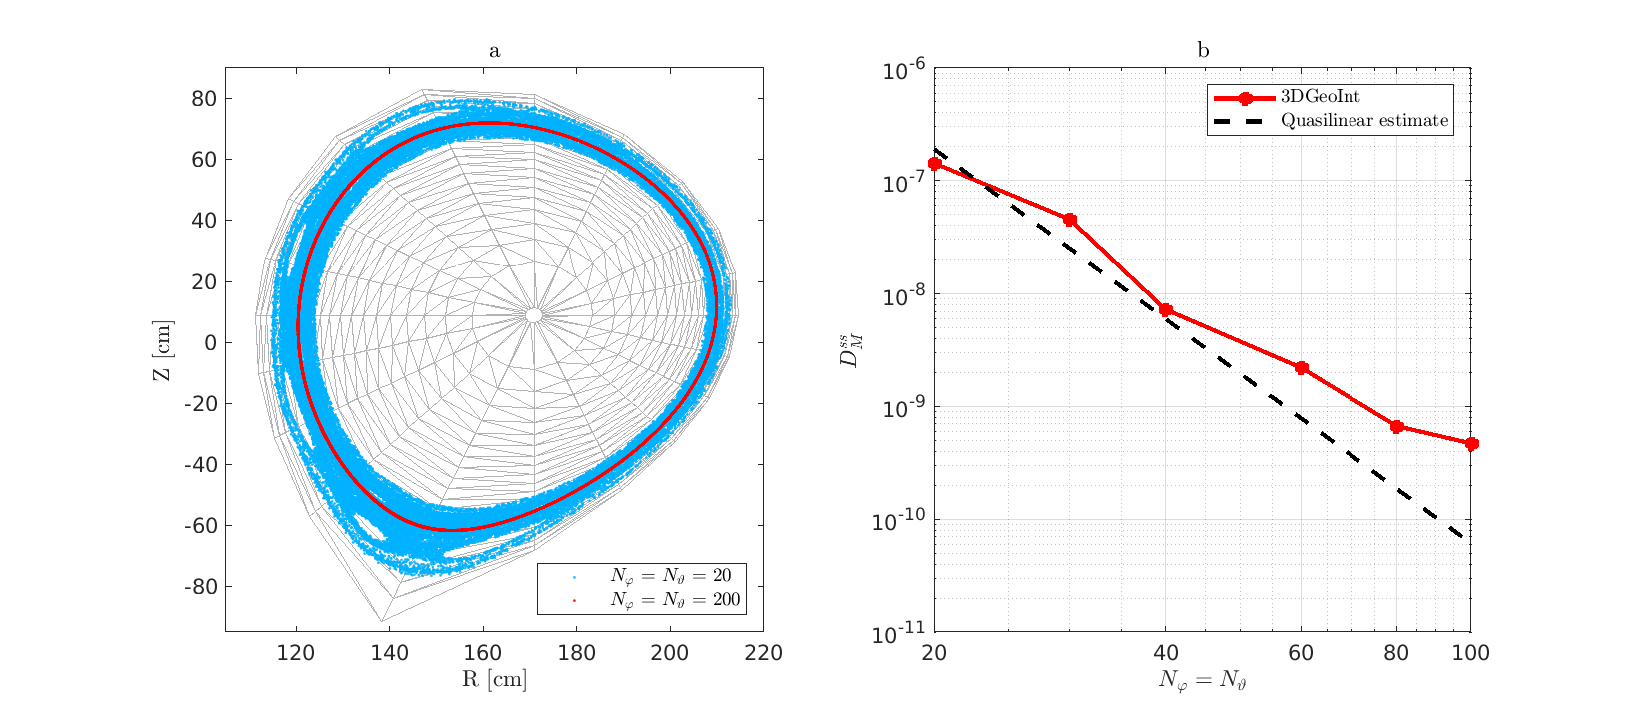
\includegraphics[width=1.25\textwidth]{FIGURES/diffusion.eps}
\end{figure}
\end{frame}



\begin{frame}
\frametitle{Artifact: Numerical field line diffusion II}
\vspace{-0.5cm}
\begin{itemize}
	\item Numerical diffusion can be put \textbf{below the level of classical electron diffusion}
	using a mild \textbf{grid refinement}.
	\item
	When tracing orbits in a \textbf{VMEC stellarator field} numerical diffusion is effectively \textbf{minimized by using symmetry flux coordinates}.
	\begin{itemize}
	\item Numerical diffusion results only from the FLR effects which lead roughly to the same
	order of perturbations as in weakly perturbed tokamaks, $\varepsilon_M \sim \rho/a$.
\end{itemize} 
	\end{itemize}
\end{frame}

\begin{frame}
\frametitle{Turning artifact into feature:}
\vspace*{-0.5cm}
\textit{\textbf{Numerical diffusion for anomalous transport modelling:}}
\begin{itemize}
	\item 3D noise in ($\vec{A}$,$\Phi$) leads to artificial diffusion.
	\item Use this diffusion as an additional transport mechanism
	to model anomalous transport.
	\item The resulting orbits are physically consistent .
	\item Adjust amplitude of the noise to reproduce phenomenological transport coefficient.
\end{itemize}

\end{frame}

\section{Application: Mono-energetic radial transport coefficient}


\begin{frame}
\frametitle{Application: Mono-energetic radial transport coefficient}
\vspace{-0.5cm}
\begin{itemize}
	\item Mono-energetic radial transport coefficient as a function of collisionality is evaluated with the Monte Carlo method.
	\item Collisions are realized by pitch angle scattering (Lorentz scattering operator).\\
	\be{}
	\frac{\partial f}{\partial t} = \frac{1}{s \left(\psi \right)} \frac{\partial}{\partial \psi}s D 	\frac{\partial f}{\partial \psi} 
	\ee
	\be{}
	D = D(E,\psi) = \langle \frac{1}{2t} \left( \psi  \left(t\right) - \psi \left( t_0 \right) \right)^2 \rangle
	\ee
\end{itemize}
\end{frame}



\begin{frame}
\frametitle{Radial Transport in HYDRA (stellarator)}
\vspace{-1.2cm}
%\hspace{-7cm}
\hspace*{0.1cm}
\begin{columns}[t]
	\begin{column}{0.8\textwidth}
		\begin{figure}
			\vspace*{-1.05cm}
\hspace*{-0.5cm}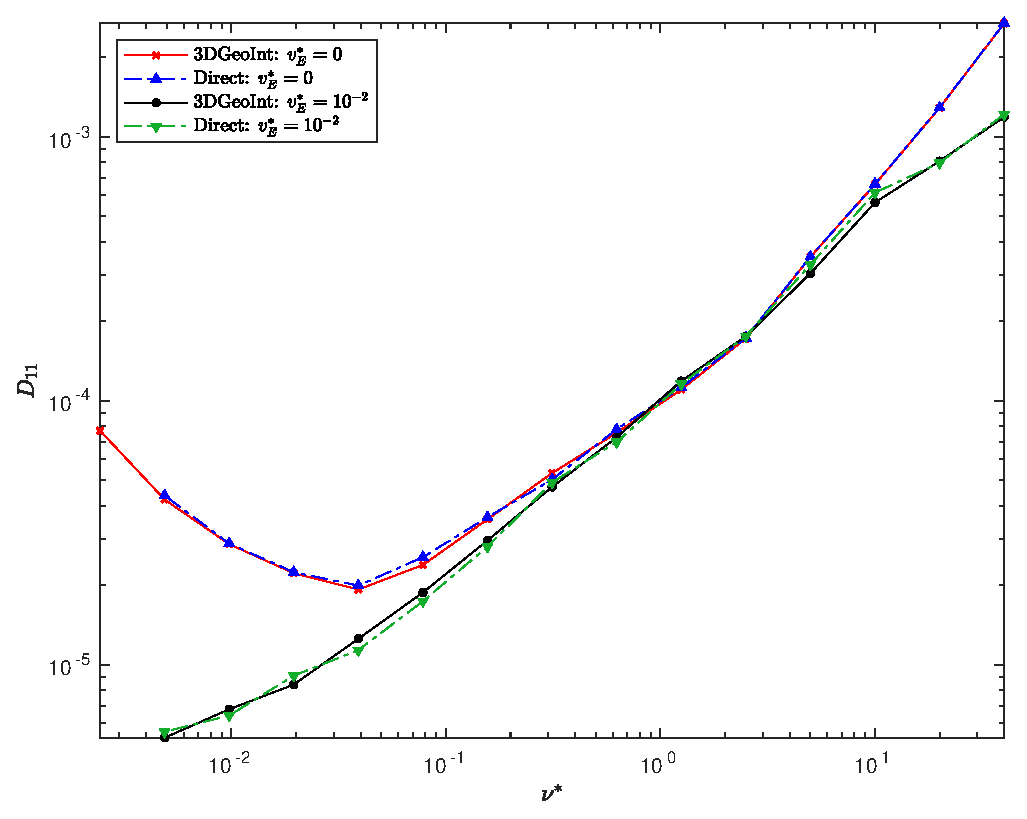
\includegraphics[width=1\textwidth]{FIGURES/transport_coefficient.eps}
\end{figure}
\end{column}
\hspace*{-1cm}
\begin{column}{0.2\textwidth}
	\vspace*{0.8cm}
	\bea*{} 
		\nu^{\ast} &=& \frac{R_0 \nu_c}{\iota v} \nonumber \\
		\quad \nonumber \\ 
		v_E^{\ast} &=& \frac{E_r}{v B_0} \nonumber
	\eea
	
	\end{column}
\end{columns}

\end{frame}


\section{Conclusion}
\begin{frame}
\frametitle{Conclusion}
\vspace*{-0.5cm}
\textit{\textbf{Advantages:}}\\
\begin{itemize}
\item Physically correct long time orbit dynamics
\item Particle coordinates and velocities are implicitly given at cell boundaries.
\item Low sensitivity to noise in electromagnetic fields
\item Computational efficiency
\end{itemize}
\textit{\textbf{Limitations:}}
\begin{itemize}
\item Artificial numerical diffusion is induced by piecewise linear field quantities.
\end{itemize}
\end{frame}

\section{Conclusion}



\section{ }
 \begin{frame}
% \frametitle{Motivation for planned\\ impurity transport modelling (2)}
% \vspace{-1mm}
% \includegraphics[width=\textwidth,height=0.8\textheight]{AUG32169_profiles}
% \begin{picture}(0,0)
% \put(0,190) {\tiny \turnbox{-90}{P. Piovesan et al, Plasma Phys. Control. Fusion 59 (2017) 014027}}
% \end{picture}
\vspace*{2.5cm}
\centerline{\huge Thank you for your attention!}
 \end{frame}



%%%%%%%%%%%%%%%%%%%%%%%%%%%%%%%%%%%%%%%%%%%%%%%%%%%%%%%%%%%%%%%%%%%%%%%%%%%%
\end{document}
%%%%%%%%%%%%%%%%%%%%%%%%%%%%%%%%%%%%%%%%%%%%%%%%%%%%%%%%%%%%%%%%%%%%%%%%%%%%

%% EOF
